\section*{Bài 4}
	
Thiết kế thuật toán Euclid để tìm ước chung lớn nhất của hai đa thức $P \big( x \big)$ và Q$\big( x \big)$ thuộc $\big[ x \big]$ (đa thức hệ số hữu tỉ). Cho ví dụ.

\begin{center}
    \textbf{\underline{Bài làm:}}
\end{center}

\begin{algorithm}
\setstretch{1.15}
\renewcommand{\algorithmcfname}{Thuật toán}

\caption{Thuật toán Euclid tìm ước chung lớn nhất của 2 đa thức}
\SetKwInOut{Input}{Đầu vào}\SetKwInOut{Output}{Đầu ra}
\SetAlgoNoEnd\SetAlgoNoLine%

\Input{Đa thức  $P \big( x \big)$ và $Q \big( x \big)$ sao cho deg$\big( P \big( x \big) \big) \geq$ deg$\big( Q \big( x \big) \big)$.}
\Output{Ước chung lớn nhất của 2 đa thức trên.}
\While{$Q \big( x \big) \neq 0$}{
    $R \big( x \big) \leftarrow \text{rem} \big( R_0, R_1 \big)$\\
    $P \big( x \big) \leftarrow Q \big( x \big)$\\
    $Q \big( x \big) \leftarrow R \big( x \big)$
}
\Return $P \big( x \big)$
\end{algorithm}

\begin{algorithm}
\setstretch{1.15}
\renewcommand{\algorithmcfname}{Thuật toán}

\caption{Thuật toán Euclid mở rộng}
\SetKwInOut{Input}{Đầu vào}\SetKwInOut{Output}{Đầu ra}
\SetKwFunction{rem}{rem}
\SetKwFunction{quo}{quo}
\SetAlgoNoEnd\SetAlgoNoLine%

\Input{Đa thức  $P \big( x \big)$ và $Q \big( x \big)$ sao cho deg$\big( P \big( x \big) \big) \geq$ deg$\big( Q \big( x \big) \big)$.}
\Output{3 đa thức $R \big( x \big), S \big( x \big), D \big( x \big)$ sao cho $R \big( x \big) \cftdot P \big( x \big) + S \big( x \big) \cftdot Q \big( x \big) = \gcd \big( P \big( x \big), Q \big( x \big) \big) = D \big( x \big)$.}
$R_0 \big( x \big) \leftarrow P \big( x \big)$\\
$U_0 \big( x \big) \leftarrow 1$\\
$V_0 \big( x \big) \leftarrow 0$\\
$R_1 \big( x \big) \leftarrow Q \big( x \big)$\\
$U_1 \big( x \big) \leftarrow 0$\\
$V_1 \big( x \big) \leftarrow 1$\\
\While{$R_1 \big( x \big) \neq 0$}{
    $T \big( x \big) \leftarrow \quo \big( R_0, R_1 \big) $\\
    $R_2 \big( x \big) \leftarrow R_0 \big( x \big) - T \big( x \big) R_1 \big( x \big)$\\
    $U_2 \big( x \big) \leftarrow U_0 \big( x \big) - T \big( x \big) U_1 \big( x \big)$\\
    $V_2 \big( x \big) \leftarrow V_0 \big( x \big) - Q \big( x \big) V_1 \big( x \big)$\\
    $U_0 \big( x \big) \leftarrow U_1 \big( x \big)$\\
    $V_0 \big( x \big) \leftarrow V_1 \big( x \big)$\\
    $R_0 \big( x \big) \leftarrow R_1 \big( x \big)$\\
    $U_1 \big( x \big) \leftarrow U_2 \big( x \big)$\\
    $V_1 \big( x \big) \leftarrow V_2 \big( x \big)$\\
    $R_1 \big( x \big) \leftarrow R_2 \big( x \big)$\\
}
\Return $U_0 \big( x \big), V_0 \big( x \big), R_0 \big( x \big)$
\end{algorithm}

\textbf{Hiện thực thuật toán trên Maple:}

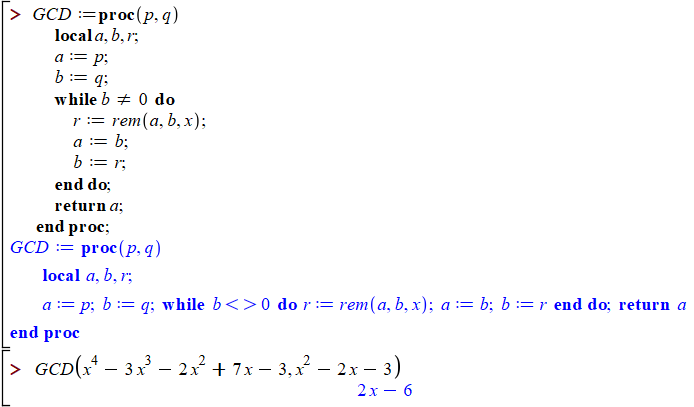
\includegraphics[width=1.0\textwidth]{bai4.png}

\addcontentsline{toc}{section}{Bài 4}

\clearpage